\documentclass[main.tex]{subfiles}
\begin{document}

\section*{Tue Dec 17 2019}

% \begin{figure}[ht]
%     \centering
%     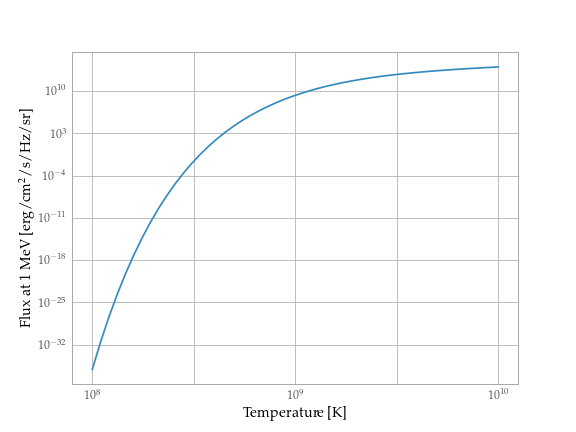
\includegraphics[width=\textwidth]{figures/flux_1_MeV.png}
%     \caption{Flux at \SI{1}{MeV} for a blackbody with varying temperature \(T\).}
%     \label{fig:flux-1-MeV}
% \end{figure}

The critical parameter governing if and how this instability gives rise to an explosion is the mass of the heavy (Helium) core.

The number of pulsation instabilties decreases as the He core mass increases.
After \(60 M_{\odot}\) only one pulsation is needed in order to blow off the whole core.

Typically the binding energies of the outer layers of very massive stars is rather low, on the order of \SI{e48}{erg} to \SI{e49}{erg}, while a pulse generally has energies of the order \SI{e49}{erg} to \SI{e51}{erg}. 

After each of these pulses, the star contracts again and the process can repeat, if the temperatures reached are high enough.
If it cannot start the pulsation again, it keeps evolving until it forms an iron core and undergoes a regular core collapse SN explosion.

The time between pulses increases dramatically as \(M _{\text{He}}\) increases; also the number of pulses decreases.

\subsection{The population of PCSNe}

People generally focus on low metallicity, very massive stars in order to study PCSNe, since we need low metallicity in order for the star not to lose too much mass and still have a massive enough He core.

So, people usually studied Population III stars, but recent developments show that even stars with a metallicity as high as \(Z_{\odot} / 3\) could be candidates for PCSN explosions; so based on stellar population models we should expect 1 supernova in \num{e5} to be a PCSN in the local universe.

The super-luminous SNe observed in the local universe could possibly be PCSNe.
% For example, they are found in the Magellanic clouds. 

Many factors affect the growth of the oxygen core: 
\begin{enumerate}
    \item the rate of the nuclear reaction \(\ce{^{12}C}(\alpha , \gamma ) \ce{^{16}O}\), which affects the C/O ratio at the end of helium burning;
    \item convective overshooting reduces the minimum mass for a PCSN to around \(100 \divisionsymbol 120M_{\odot}\);
    \item rotation-induced chemical mixing also reduces the minimum stellar mass needed in order to have a PCSN;
    \item rotation decreases the binding energy: it increases the maximum mass needed in order to have a PCSN.
\end{enumerate}

\subsection{Pair Creation Supernovae: the dynamics of the explosion}

If \(60 M_{\odot} \lesssim  M _{\text{He}} \lesssim 130M_{\odot}\) a single pulse can completely disrupt the star. 

Plots of the nuclear binding, gravitational binding and kinetic energies are useful to understand the process. 

As soon as carbon burning ends, the nuclear binding energy sharply decreases because of explosive O and Si burning, making the star globally unbound. 

The kinetic energy released by the explosion of a star with a global mass of \(250M_{\odot}\) is of the order of \SI{44}{foe}; the ejected material reaches asymptotic velocities of the order \(\num{.017}c\).

\subsection{Chemical Yields of the explosion}

% The nuclear front crosses the various layers of the star. 
If we increase the initial mass of the star, the amount of Nickel produced increases: let us fix the metallicity as \(Z = \num{.001}\); then, if the starting mass is \(M = 150M_{\odot}\) then the Nickel mass produced is \(\num{.04}M_{\odot}\); if the starting mass is \(M = 250M_{\odot}\) then the Nickel mass produced is \(\num{19.3}M_{\odot}\).

We can plot the production factor of various nuclides relative to the solar rate of production: as the isotope charge number varies: we plot \(\log (\text{prod} / \text{solar prod})\).
If the starting metallicity of the star increases, the production rate of these elements decreases.
Also, if the starting mass of the star increases these yields increase.

We see a zig-zag pattern: a large difference between even and odd nuclides,
% Even nuclides are produced more (since all of the nuclides start out from \(\alpha = \ce{^{4}He} \), this makes sense). 
even nuclides are produced more.
This is because of the lack of neutrons, which is quantified by the neutron excess parameter: 
%
\begin{align}
\eta = \sum _{i} \frac{(N_i - Z_i)X_i}{A_i}
\,;
\end{align}
%
in PCSNe \(\eta \) is lower than in CCSNe, since 
the cores of the stars undergoing PCSN explosions are much less dense than those undergoing CCSN explosions, so neutronization is much less relevant.

Lots of Oxygen is left unburnt and thus is ejected in the explosion.

The amount of ejected material beyond iron is low. 

The production of Nickel, mentioned above, is important because of the decay chain \(\ce{Ni} \rightarrow \ce{Co} \rightarrow \ce{Fe}\), which could explain the shape of the decaying light curve of the supernova.

The reactions, more specifically, are 
%
\begin{align}
\ce{^{56}Ni} + e^{-} &\rightarrow \ce{^{56}Co} + \nu + \gamma  && t_{1/2} \approx \SI{6.1}{d}   \\
\ce{^{56}Co} + e^{-} &\rightarrow \ce{^{56}Fe} + \nu + \gamma && t_{1/2} \approx \SI{77}{d} 
\,,
\end{align}
%
which matches well the exponentially decaying light curve after \(50 \divisionsymbol \SI{100}{d}\).

This constrains the amount of Nickel produced: for the lightcurves of CCSNe it is around \(\num{.07}M_{\odot}\).

\subsection{PISN and PCSN contribution to the chemical evolution of galaxies}

We want to invesigate how relevant these SN explosions are for the chemical composition of low-metallicity galaxies, with metallicities around \(Z_{\odot} / 3 \divisionsymbol Z_{\odot} / 10\), below the PISN critical metallicity. 

\todo[inline]{I think this is what was meant, but I'm not sure about it. The slide seemed to imply that the critical metallicity for PISN \emph{is} \(Z_{\odot} /3 \) to \(Z_{\odot} / 10\), which does not seem right.}

In order to study this, we need to know how many PISN progenitors (i.e.\ very massive stars) form per unit time.
They can be created as a result of very rapid mass accretion, or after mergers in binary star systems, or from stellar collisions.

The mass distribution of stars is not well known, an educated guess is a Salpeter-like mass function, \(\varphi (M) \dd{m} \sim M^{-2.5} \dd{m}\).
If we assume this, we predict that around \SI{2}{\percent} of supernova explosions should be massive enough to form a PISN.

We can plot the metal yield multiplied by the probability to have a star of that mass as the mass of the star varies: this models the total contribution to the metallicity in the ISM of that specific mass range. 

We include Core Collapse SNe (with \(M < 50 M_{\odot}\)), then there is a mass region in which mostly BHs are formed, and then we have PISNe from \(120 M_{\odot}< M < 260 M_{\odot}\), then BHs again. 

The total mass yield per unit initial mass is lower for PISNe than for CCSNe, but the mass range is larger so the total yields of the two types of supernova explosion are comparable.

\paragraph{Per-element yields}

We compare the per-element yields of four different models:
\begin{enumerate}
    \item CCSN alone at \(Z=0\);
    \item CCSN + PCSN at \(Z=0\);
    \item CCSN alone at \(Z=\num{.002}\);
    \item CCSN at \(Z = \num{.002}\) + PCSN at \(Z=\num{.001}\).
\end{enumerate}

We notice the following things when considering the heavy (after Oxygen) elements: 
\begin{enumerate}
    \item at higher metallicity the yields are in general higher;
    \item we always see an even-odd effect, with even elements being produced more, and
    \item this effect is less pronounced if we only look at CCSNe;
    \item this effect is less pronounced at higher metallicity.
    \item The production of elements after Iron is not dependent on the metallicity, and their production is negligible in PCSNe.
\end{enumerate}

\subsection{PCSNe light curves}

We can model the light curves by simply solving the hydrodinamical and radiative transport equations.

The bolometric magnitude light curve follows the visual curve for a certain time period, before which it needs UV corrections, and after which it needs IR corrections.

% Partial test on the 14th of January.

\end{document}